\part{Estrutura Analítica do Projeto}
\chapter[Estrutura Analítica do Projeto]{Estrutura Analítica do Projeto}

No gerenciamento de projeto, A ESTRUTURA ANALÍTICA DO PROJETO (EAP) ou em inglês WORKBREAkDOWN STRUCTURE é uma ferramenta de subdivisão das entregas e trabalhos do projeto em componentes menores, facilitando o gerenciamento.

Na EAP do projeto SmartGrid, inicialmente foi divido em três sub categorias que seriam ela os pontos de controles, sendo que a parti dessas categorias foi quebrando as metas e trabalhos que deveriam ser realizados para que o projeto tenha êxito, e que facilite o gerenciamento. 

Sendo uma das principais entregas do primeiro ponto de controle, seria mostra as problemáticas que o projeto pretende solucionarem. De mostrando a importância da implementação do projeto (SmartGrid). No segundo ponto de controle a principal entrega, será a da solução dos problemas que foram apresentados no ponto de controle 1. O ponto de controle três, já traz como sua entrega principal, a visão econômica do projeto e sua viabilidade, seu rendimento e tempo de retorno do investimento.

A figura \ref{fig:eap} apresenta a estrutra analítica do projeto em questão

\begin{figure}[!h]
	\centering
	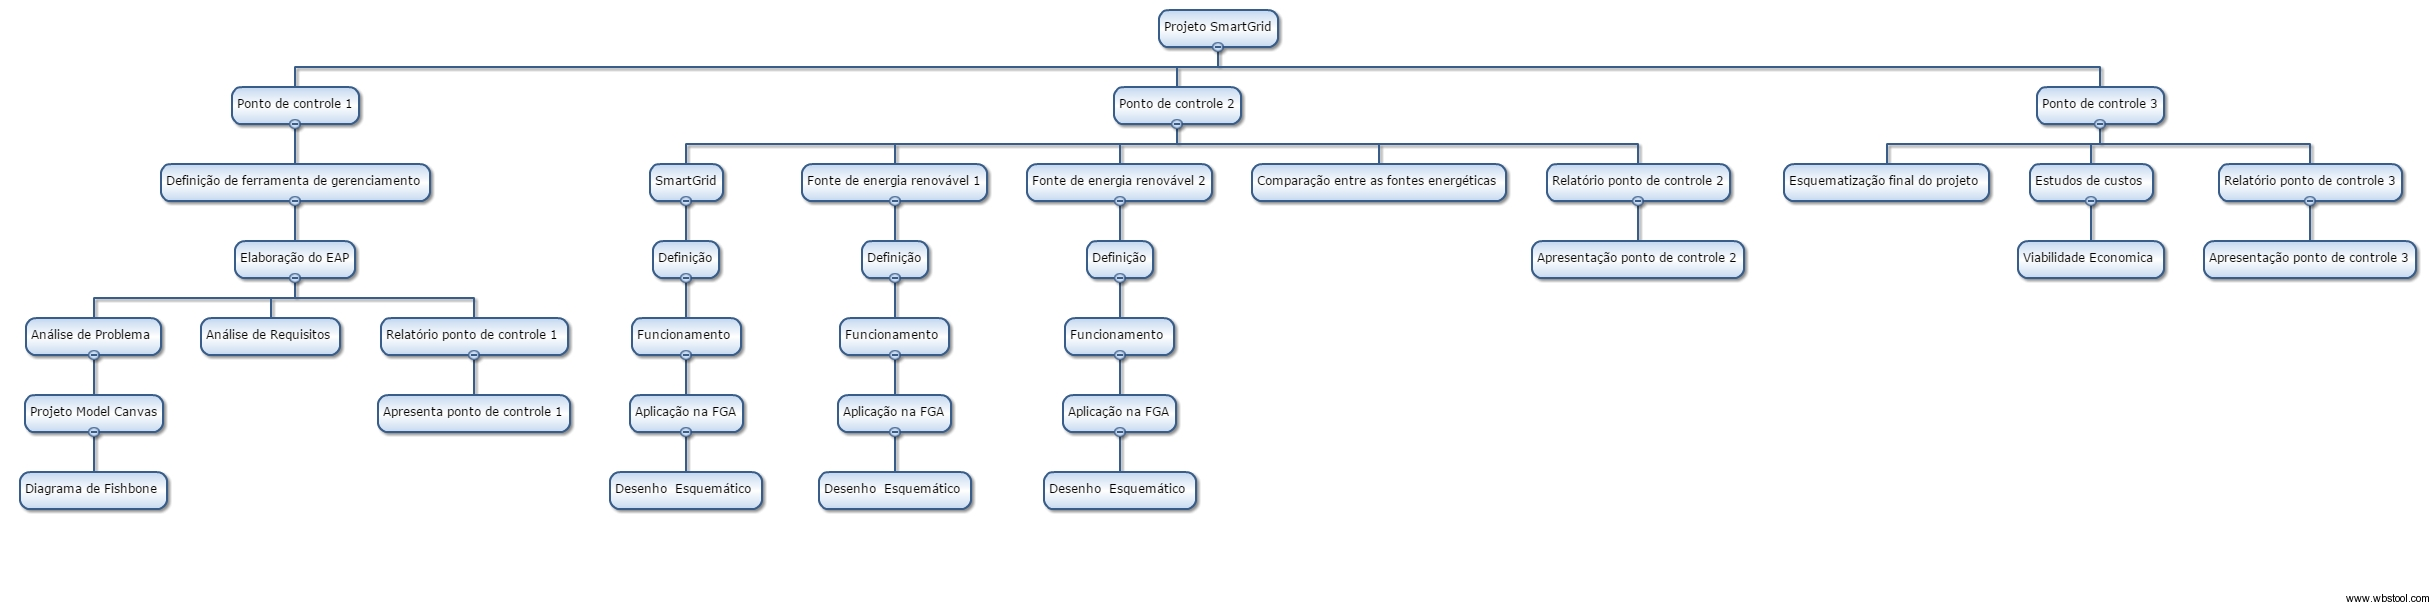
\includegraphics[angle=270, scale=.3]{figuras/EAP.jpg}
	\caption{Estrutura Analítica do projeto SmartGrid para a FGA}
	\label{fig:eap}
\end{figure}